\section{Технический проект}
\subsection{Общая характеристика организации решения задачи}

Для эффективного управления энергопотреблением в зданиях предлагается разработать комплексную программно-информационную систему, в основе которой лежат передовые технологии. Создаваемая система будет включать в себя несколько ключевых модулей, в том числе модули мониторинга, управления, аналитики и интеграции с внешними устройствами.

Модуль мониторинга будет ответственен за сбор и анализ данных об энергопотреблении в режиме реального времени. Это позволит системе непрерывно отслеживать изменения в расходе энергии и выявлять потенциальные области оптимизации. Модуль управления предоставит пользователям средства активного воздействия на энергопотребление, позволяя оптимизировать его в соответствии с текущими потребностями и требованиями.

Особое внимание будет уделено модулю аналитики, который обеспечит глубокий анализ данных и выделение основных трендов в потреблении энергии. Это позволит пользователям принимать информированные решения для дальнейшей оптимизации и снижения затрат. Система также будет способна интегрироваться с различными внешними устройствами и системами, обеспечивая максимальную гибкость и совместимость.

Проектная цель заключается в предоставлении пользователям возможности не только наблюдать за энергопотреблением, но и активно вмешиваться в процессы управления, с целью обеспечения оптимальной эффективности и экономии ресурсов. Разрабатываемая система ставит своей задачей создание интеллектуального и адаптивного подхода к управлению энергопотреблением, способного эффективно реагировать на изменяющиеся условия и потребности.

\subsection{Обоснование выбора технологии проектирования}

Выбор языка программирования и фреймворка - критический этап в проектировании программно-информационных систем. Для разработки системы управления энергопотреблением в зданиях был принят решительный выбор в пользу языка программирования Python с использованием фреймворка Django. Этот выбор обоснован рядом значимых преимуществ, которые существенно повысят эффективность и надежность проекта.

В первую очередь, Python предоставляет высокую степень читаемости кода и простоты синтаксиса, что облегчает понимание и совместную работу над проектом. Это особенно важно в контексте разработки программных продуктов, где четкость кода и удобство его поддержки играют ключевую роль.

Фреймворк Django, в свою очередь, предоставляет набор готовых инструментов и абстракций, спроектированных для ускорения процесса разработки. Модульность, встроенная система аутентификации, ORM (Object-Relational Mapping) для удобной работы с базой данных – все это делает Django мощным инструментом для создания сложных и надежных веб-приложений.

Дополнительно, обширное сообщество разработчиков Python и Django предоставляет широкий спектр готовых решений, библиотек и обновлений, что обеспечивает высокую поддержку и стабильность проекта на протяжении его жизненного цикла.

Такой сбалансированный выбор технологий, основанный на надежности, удобстве разработки и поддержке, позволяет ожидать успешную реализацию программно-информационной системы и обеспечивает ее легкость в последующем масштабировании и совершенствовании.

\subsubsection{Описание используемых технологий и языков программирования}

Язык программирования Python является краеугольным камнем нашего проекта, обусловленного несколькими ключевыми характеристиками. Прежде всего, простота синтаксиса Python и его высокая читаемость способствуют более эффективной разработке и сопровождению кода. Это особенно важно для проектов, направленных на веб-разработку, где четкость и легкость восприятия кода имеют первостепенное значение.

Выбор фреймворка Django обусловлен его мощью и удобством использования. Django предоставляет разработчикам набор инструментов, включая систему управления базой данных, встроенные механизмы аутентификации и авторизации, а также мощный движок для обработки URL-запросов. Это позволяет сфокусироваться на бизнес-логике приложения, ускоряя процесс разработки и повышая его надежность.

Одним из важных компонентов выбора технологии стало применение Object-Relational Mapping (ORM) в Django. ORM обеспечивает абстракцию базы данных от языка SQL, что упрощает взаимодействие с данными и позволяет разработчикам оперировать объектами в коде, а не прямо с SQL-запросами. Это не только уменьшает вероятность ошибок, связанных с базой данных, но и делает код более чистым и легко поддерживаемым.

Таким образом, выбор Python и Django, а также использование ORM, формируют сбалансированный стек технологий, обеспечивая эффективную и устойчивую основу для разработки программно-информационной системы управления энергопотреблением в зданиях.

\subsubsection{Язык программирования Python Django}

Выбор языка программирования Python с применением фреймворка Django оказался стратегически обоснованным для разработки программно-информационной системы по управлению энергопотреблением в зданиях. Этот выбор основывается на ряде ключевых преимуществ, которые содействуют эффективной и надежной реализации поставленных задач.

1. Простота и Читаемость Кода: Python славится своей простотой синтаксиса, что ускоряет процесс разработки и облегчает понимание кода. Это особенно ценно для командной работы и последующего сопровождения программы.

2. Широкое Применение в Веб-Разработке: Python является одним из наиболее популярных языков программирования в области веб-разработки. Его использование с фреймворком Django обеспечивает высокую производительность и удобство для создания сложных веб-приложений.

3. Гибкость и Мощь Django: Django предоставляет разработчикам удобные инструменты, встроенные решения и структуру проекта, что упрощает создание масштабируемых и надежных приложений. Фреймворк включает механизмы для работы с базой данных, управления пользователями, обработки форм и другие полезные функции.

4. Активное Сообщество и Поддержка: Используя Python с Django, проект получает поддержку от активного сообщества разработчиков. Это обеспечивает доступ к обширным ресурсам, библиотекам и решениям, способствуя более быстрой и безопасной разработке.

5. Объектно-Реляционное Отображение (ORM): Применение ORM в Django упрощает взаимодействие с базой данных, предоставляя абстракцию от языка SQL. Это повышает безопасность и чистоту кода, делая его более поддерживаемым.

Общий результат - это мощный и гибкий инструментарий, способствующий созданию высокоэффективной программно-информационной системы, специально нацеленной на управление энергопотреблением в зданиях.

\subsection{Диаграмма компонентов}

Диаграмма компонентов – это визуальное представление структуры программной системы, выделяя её основные компоненты и взаимосвязи между ними. Она служит инструментом для понимания архитектуры приложения.

Схема обмена данными дополняет диаграмму компонентов, демонстрируя, как информация передается между различными компонентами системы. Это важный элемент, который помогает лучше понять взаимодействие между частями приложения.

На рисунке ~\ref{compnew:image} представлена диаграмма компонентов, на которой наглядно изображены основные элементы программной системы и их взаимосвязи. 

%\begin{figure}[ht]
%	\center{\includegraphics[width=1\linewidth]{compnew}}
%	\caption{Диаграмма компонентов}
%	\label{compnew:image}
%\end{figure}


\begin{landscape}
	
	\begin{плакат}
		\includegraphics[width=0.82\linewidth]{compnew}
		\caption{Диаграмма компонентов}
		\label{compnew:image}      
	\end{плакат}
\end{landscape}

Эта визуализация позволяет разработчикам и другим участникам проекта легче ориентироваться в структуре приложения и эффективнее взаимодействовать при работе над проектом.

Каталоги:
\begin{enumerate}
\item /templates/:
\begin{itemize}
\item Описание: Содержит файлы шаблонов HTML для веб-интерфейса.
\end{itemize}

\item /static/:
\begin{itemize}
\item Описание: Хранит статические файлы, такие как CSS, JavaScript, изображения.
\end{itemize}

\end{enumerate}


Компоненты:
\begin{enumerate}
	
\item Web Interface (Веб-интерфейс)

\begin{itemize}
\item Описание: Компонент, предоставляющий пользовательский интерфейс через веб-браузер.
Файлы: templates/, static/
\end{itemize}

\item Backend Server (Серверное приложение)
\begin{itemize}
\item Описание: Компонент, обрабатывающий логику приложения и предоставляющий API для взаимодействия с фронтендом.
\item Файлы: views.py, models.py, urls.py
\end{itemize}

\item Database (База данных)
\begin{itemize}
\item Описание: Компонент, отвечающий за хранение данных.
\item Файлы: Миграции Django, models.py
\end{itemize}

\item Settings (Настройки)
\begin{itemize}
\item Описание: Компонент, содержащий настройки Django, такие как подключение к базе данных, ключи и другие конфигурационные параметры.
\item Файлы: settings.py
\end{itemize}

\item Django ORM (Объектно-реляционное отображение)
\begin{itemize}
\item Описание: Компонент, предоставляющий интерфейс для взаимодействия с базой данных через Django.
\item Файлы: Встроенные Django-модели
\end{itemize}

\item Data Reading Algorithm (Алгоритм считывания данных)
\begin{itemize}
\item Описание: Компонент, включающий алгоритмы считывания данных с устройств, таких как сенсоры, датчики влажности, температуры и другие. Отвечает за обработку данных, полученных от физических устройств, и передачу их в систему для дальнейшей обработки.
\item Файлы: {alg.py}
\end{itemize}



\end{enumerate}







%\vspace{32mm} % чтобы убрать пустую строку, которая осталась после переноса рисунка на следующую страницу
%\vspace{16mm}
%\begin{figure}[ht]
%	\center{\includegraphics[width=0.89\linewidth]{comp22}}
%	\caption{Диаграмма компонентов}
%	\label{comp22:image}
%\end{figure}

%\vspace{32mm}
%\vspace{16mm} % чтобы убрать пустую строку, которая осталась после переноса рисунка на следующую страницу


%\begin{figure}[ht]
%	\center{\includegraphics[width=0.89\linewidth]{comp33}}
%	\caption{Диаграмма компонентов}
%	\label{comp33:image}
%\end{figure}
%\vspace{-8mm} % чтобы убрать пустую строку, которая осталась после переноса рисунка на следующую страницу


\begin{comment}

На диаграмме компонентов выделены следующие основные компоненты views.py:
\begin{itemize}
\item \textbf{home} - Обработчик отображения домашней страницы.

Parameters:
- request: объект запроса Django.

Returns:
- Получает данные о текущем пользователе из запроса.
- Формирует контекст с данными о пользователе.
- Возвращает страницу домашней страницы с переданным контекстом.

Возвращаемый шаблон:
- 'AC/Home/home-ac.html'.

Контекст:
- 'user': Объект текущего пользователя.

\item \textbf{create-company} - Обработчик создания новой компании.

Parameters:
- request: объект запроса Django.

Returns:
- Если метод запроса POST:
- Получает данные из формы создания компании.
- Если форма валидна, сохраняет новую компанию.
- Перенаправляет на домашнюю страницу.
- Если метод запроса GET:
- Создает форму для создания компании.
- Возвращает страницу с формой создания компании.

Возвращаемый шаблон:
- Если метод запроса GET или POST:
- 'AC/Admin/add-company-ac.html'.

Контекст:
- 'form': Экземпляр формы создания компании.

\item \textbf{delete-company} - Обработчик удаления компании.

Parameters:
- request: объект запроса Django.
- company-id: идентификатор компании, которую нужно удалить.

Returns:
- При успешном удалении компании:
- Перенаправляет пользователя на домашнюю страницу.
- Если компания не найдена:
- Возвращает страницу с ошибкой 404.


\item \textbf{create-object} - Обработчик создания нового объекта.

Parameters:
- request: объект запроса Django.

Returns:
- Если метод запроса POST:
- Получает данные из формы создания объекта.
- Если форма валидна, сохраняет новый объект.
- Перенаправляет на домашнюю страницу.
- Если метод запроса GET:
- Создает форму для создания объекта.
- Возвращает страницу с формой создания объекта.

Возвращаемый шаблон:
- Если метод запроса GET или POST:
- 'AC/Admin/add-object-ac.html'.

Контекст:
- 'form': Экземпляр формы создания объекта.

\item \textbf{create-object-to-room} - Обработчик создания нового объекта в комнате.

Parameters:
- request: объект запроса Django.

Returns:
- Если метод запроса POST:
- Получает данные из формы создания объекта в комнате.
- Если форма валидна, сохраняет новый объект в комнате.
- Перенаправляет на домашнюю страницу.
- Если метод запроса GET:
- Создает форму для создания объекта в комнате.
- Возвращает страницу с формой создания объекта в комнате.

Возвращаемый шаблон:
- Если метод запроса GET или POST:
- 'AC/Admin/add-object-to-room-ac.html'.

Контекст:
- 'form': Экземпляр формы создания объекта в комнате.


\item \textbf{create-room} - Обработчик создания новой комнаты.

Parameters:
- request: объект запроса Django.

Returns:
- Если метод запроса POST:
- Получает данные из формы создания комнаты.
- Если форма валидна, сохраняет новую комнату.
- Перенаправляет на домашнюю страницу.
- Если метод запроса GET:
- Создает форму для создания комнаты.
- Возвращает страницу с формой создания комнаты.

Возвращаемый шаблон:
- Если метод запроса GET или POST:
- 'AC/Admin/add-room-ac.html'.

Контекст:
- 'form': Экземпляр формы создания комнаты.

\item \textbf{profile} -Обработчик отображения профиля пользователя.

Parameters:
- request: объект запроса Django.

Returns:
- Получает данные пользователя по его идентификатору из запроса.
- Формирует контекст с данными пользователя.
- Возвращает страницу профиля с переданным контекстом.

Возвращаемый шаблон:
- 'AC/Profile/profile-ac.html'.

Контекст:
- 'user': Объект пользователя с данными профиля.

\item \textbf{update-profile} -  Обработчик обновления профиля пользователя.

Parameters:
- request: объект запроса Django.

Returns:
- Если метод запроса POST:
- Получает данные из формы обновления профиля пользователя.
- Если форма валидна, сохраняет обновленные данные профиля.
- Перенаправляет на страницу профиля.
- Если метод запроса GET:
- Создает форму для редактирования профиля с данными текущего пользователя.
- Возвращает страницу с формой редактирования профиля.

Возвращаемый шаблон:
- Если метод запроса GET или POST:
- 'AC/Profile/edit-profile-ac.html'.

Контекст:
- Если метод запроса GET:
- 'form': Экземпляр формы редактирования профиля с данными текущего пользователя.

\item \textbf{change-password} - Обработчик изменения пароля пользователя.

Parameters:
- request: объект запроса Django.

Returns:
- Если метод запроса POST:
- Получает новый пароль из формы.
- Устанавливает новый пароль для текущего пользователя.
- Сохраняет изменения и обновляет хэш аутентификации в сессии.
- Перенаправляет на страницу профиля.
- Если метод запроса GET:
- Возвращает страницу с формой изменения пароля.

Возвращаемый шаблон:
- Если метод запроса GET или POST:
- 'AC/Profile/forgotyourpassword-ac.html'.

\item \textbf{reset-password} -     Обработчик сброса пароля пользователя.

Parameters:
- request: объект запроса Django.

Returns:
- Если метод запроса POST:
- Получает имя пользователя из формы.
- Пытается найти пользователя с указанным именем.
- Если пользователь найден, устанавливает новый пароль 'qwerty123' и сохраняет изменения.
- Перенаправляет на страницу входа.
- Если пользователь с указанным именем не найден, обработывает исключение User.DoesNotExist.
- Если метод запроса GET:
- Возвращает страницу сброса пароля.

Возвращаемый шаблон:
- Если метод запроса GET:
- 'AC/Profile/forgotyourpassword-ac.html'.
- Если метод запроса POST:
- Нет.

\item \textbf{delete-profile} - Обработчик удаления профиля пользователя.

Parameters:
- request: объект запроса Django.

Returns:
- Если метод запроса POST:
- Получает текущего пользователя.
- Удаляет профиль пользователя.
- Выполняет выход пользователя из системы.
- Перенаправляет на страницу входа.
- Если метод запроса GET:
- Возвращает страницу подтверждения удаления профиля.

Возвращаемый шаблон:
- Если метод запроса GET:
- 'AC/Profile/delete-profile-ac.html'.
- Если метод запроса POST:
- Нет.

\item \textbf{register} - Обработчик регистрации пользователей.

Parameters:
- request: объект запроса Django.

Returns:
- Если метод запроса POST:
- Если данные формы валидны, создается новый пользователь с использованием данных из формы.
- Выполняется вход в систему от имени нового пользователя.
- Перенаправляет на страницу профиля.
- Если метод запроса GET:
- Создает экземпляр формы регистрации.
- Рендерит страницу регистрации с пустой формой.

Возвращаемый шаблон:
- 'AC/Profile/registration-ac.html'

Контекст:
- 'form': Экземпляр формы регистрации.

\item \textbf{login-view} - Обработчик входа пользователя в систему.

Parameters:
- request: объект запроса Django.

Returns:
- Если метод запроса POST:
- Проверяет переданные учетные данные пользователя с использованием Django's authentication system.
- Если учетные данные верны, выполняет вход пользователя в систему и перенаправляет на страницу профиля.
- В противном случае, возвращает страницу входа с сообщением об ошибке.
- Если метод запроса GET:
- Возвращает страницу входа.

Возвращаемый шаблон:
- Если метод запроса POST и учетные данные неверны:
- 'AC/Profile/login-ac.html' с переданным сообщением об ошибке.
- В остальных случаях:
- 'AC/Profile/login-ac.html'.

Контекст:
- Если метод запроса POST и учетные данные неверны:
- 'error-message': Сообщение об ошибке для отображения на странице входа.

\item \textbf{logout-view} - Обработчик выхода пользователя из системы.

Parameters:
- request: объект запроса Django.

Returns:
- Выполняет выход текущего пользователя из системы.
- Перенаправляет на страницу входа.

\item \textbf{floor-view} - Обработчик отображения этажа с комнатами.

Parameters:
- request: объект запроса Django.

Returns:
- Получает номер этажа из параметра запроса или устанавливает значение по умолчанию (1).
- Вычисляет предыдущий и следующий этажи.
- Пытается получить объект этажа по номеру.
- Если объект этажа существует, получает комнаты на этом этаже.
- Формирует контекст с данными о текущем этаже, предыдущем и следующем этажах, а также списком комнат.
- Возвращает страницу с информацией об этаже и комнатах или страницу ошибки 404, если этаж не найден.

Возвращаемый шаблон:
- Если этаж найден:
- 'AC/floors.html'.
- Если этаж не найден:
- 'AC/404.html'.

\item \textbf{energy-consumption-chart} -     Получение данных о потреблении энергии для компании.

Parameters:
- company-id: Идентификатор компании.

Returns:
- months: Список месяцев.
- consumption-without-assistant: Суммарное потребление электроэнергии без использования умного помощника.
- consumption-with-assistant: Суммарное потребление электроэнергии с использованием умного помощника.


\item \textbf{cabinet-view} -     Обработчик отображения информации о кабинете (комнате).

Parameters:
- request: объект запроса Django.
- floor: Номер этажа.
- cab-num: Номер кабинета.

Returns:
- Если кабинет найден:
- Получает данные о кабинете, инвентаризации и потреблении энергии.
- Формирует контекст с данными о кабинете, предыдущем и следующем кабинетах, месяцах и потреблении энергии.
- Возвращает страницу с информацией о кабинете.
- Если кабинет не найден:
- Возвращает страницу ошибки 404.


\item \textbf{dashboard-sensors-view} - Обработчик отображения данных по датчикам и потреблению энергии для определенной компании и комнаты в определенную дату.

Parameters:
- request: объект запроса Django.
- company: Идентификатор компании (предприятия).
- room: Идентификатор комнаты.

Returns:
- Если данные существуют для указанной компании, комнаты и даты:
- Получает данные из модели EnergyConsumption.
- Формирует контекст с полученными данными и предыдущей и следующей датами.
- Возвращает страницу с отображением данных по датчикам и потреблению энергии.
- Если данных не существует:
- Возвращает страницу ошибки 404.

Возвращаемый шаблон:
- 'AC/dashboard-sensors.html' в случае успешного нахождения данных.
- 'AC/404.html' в случае отсутствия данных.

Контекст:
- 'id': Идентификатор записи.
- 'company': Компания (предприятие).
- 'room': Комната.
- 'date': Дата.
- 'consumption-without-an-assistant': Потребление энергии без использования умного помощника.
- 'consumption-with-an-assistant': Потребление энергии с использованием умного помощника.
- 'total-amount-of-electricity-consumed-without-an-assistant': Общее потребление электроэнергии без использования умного помощника.
- 'total-amount-of-electricity-consumed-with-the-assistant': Общее потребление электроэнергии с использованием умного помощника.
- 'total-cost-without-an-assistant': Общая стоимость электроэнергии без использования умного помощника.
- 'total-cost-with-an-assistant': Общая стоимость электроэнергии с использованием умного помощника.
- 'humidity': Влажность.
- 'temperature': Температура.
- 'illumination': Освещенность.
- 'motion': Наличие движения.
- 'prev-date': Предыдущая дата.
- 'next-date': Следующая дата.

\end{itemize}

\end{comment}


\subsubsection{Описание настройки Django}

Настройка Django в проекте осуществляется через два ключевых файла: settings.py и urls.py. В этих файлах определена конфигурация приложения, включая параметры базы данных, пути к шаблонам, обработку статических файлов и другие настройки. В settings.py размещаются параметры, определяющие общую конфигурацию проекта, такие как настройки базы данных, приложения, подключение статических и медиа файлов, а также многое другое. С другой стороны, в urls.py определяются пути маршрутизации, которые связывают URL-адреса с соответствующими представлениями и функциональностью приложения. Эти два файла играют ключевую роль в формировании и управлении всеми аспектами функционирования Django-приложения, обеспечивая его корректное взаимодействие с веб-сервером и клиентскими запросами.
 
\paragraph{База данных}

Один из важных аспектов Django-проекта – это выбор и настройка системы управления базами данных (СУБД). В данном случае, в качестве СУБД используется PostgreSQL, предоставляющая надежное и мощное хранилище данных.

Для интеграции PostgreSQL в Django проект, первоначально необходимо установить соответствующий пакет драйвера, в данном случае, psycopg2. Этот драйвер обеспечивает связь между Django и PostgreSQL, обеспечивая эффективное взаимодействие с базой данных.

После установки драйвера, производится конфигурация подключения к базе данных в файле settings.py. Здесь определяются параметры, такие как имя базы данных, пользователь, пароль, хост и порт, необходимые для успешного соединения с PostgreSQL. Это обеспечивает правильную интеграцию между Django приложением и выбранной базой данных, что является фундаментом для эффективного хранения и обработки данных в рамках проекта. Пример настройки:

 
\begin{lstlisting}[language=Python]
DATABASES = {
	'default': {
		'ENGINE': 'django.db.backends.postgresql',
		'NAME': 'mydatabase',
		'USER': 'mcherenkov',
		'PASSWORD': '*2nm(h(tIs2u4AJ#',
		'HOST': 'localhost',
		'PORT': '5432',
	}
}
\end{lstlisting}  
 
Эти параметры включают в себя имя базы данных, пользователя, пароль, хост и порт для подключения к PostgreSQL.

\paragraph{Статические файлы и медиа}

Настройки для обработки статических файлов и медиа файлов (например, изображений, загружаемых пользователями) также определены в settings.py. Важным аспектом конфигурации Django-проекта является определение параметров обработки статических и медиа файлов. Эти файлы могут включать в себя стили, скрипты, изображения, а также медиа-контент, загружаемый пользователями.
 
Такие настройки позволяют эффективно управлять статическими и медиа-ресурсами в Django-проекте, обеспечивая их доступность и корректное отображение на веб-страницах.Пример настроек для статических файлов:
 
\begin{lstlisting}[language=Python]
STATIC_URL = '/static/'
STATICFILES_DIRS = [BASE_DIR / "static"]

MEDIA_URL = '/media/'
MEDIA_ROOT = BASE_DIR / "media"

\end{lstlisting}  

Здесь STATIC-URL указывает префикс для статических файлов, а STATICFILES-DIRS - на каталог, где хранятся эти файлы.

MEDIA-URL и MEDIA-ROOT аналогичны, но используются для обработки медиа файлов.

\paragraph{Настройки безопасности}

Django также предоставляет настройки безопасности, такие как секретный ключ, список разрешенных хостов (ALLOWED-HOSTS), и другие параметры. Пример:

 
\begin{lstlisting}[language=Python]
SECRET_KEY = 'django-insecure-b)te6480y4j&yunr@zy6v#$2u(r@06q3kb$m@=d1n!_8t&(xj!'
DEBUG = False
ALLOWED_HOSTS = ['mcherenkov.com']
\end{lstlisting} 
 
Секретный ключ должен быть уникальным и долгим случайным значением. Включение параметра DEBUG в режиме разработки может быть удобным для поиска ошибок, но необходимо отключить его в продакшн окружении. Список разрешенных хостов (ALLOWED-HOSTS) определяет, какие хосты могут обращаться к вашему серверу. 

 
\subsection{Диаграмма размещения}
\begin{comment}
	

Для создания диаграммы размещения, нам нужно учитывать архитектурные компоненты программной системы и то, как они будут размещены на физических устройствах. Ниже представлен пример общей структуры диаграммы размещения для "Программно-информационная система для управления энергопотреблением в зданиях". В диаграмме должны быть представлены следующие элементы:
\end{comment}

При проектировании диаграммы размещения необходимо тщательно рассмотреть взаимодействие архитектурных компонентов программной системы и их распределение по физическим устройствам. Эффективное размещение данных компонентов определяет стабильность и производительность системы. Приведенный ниже пример диаграммы размещения является иллюстрацией общей структуры "Программно-информационной системы для управления энергопотреблением в зданиях", включающей в себя ключевые элементы, начиная от клиентских устройств и заканчивая устройствами управления энергопотреблением в физических зданиях.

Серверная инфраструктура, показывает сервера, на которых размещаются серверные компоненты системы, такие как веб-сервер, базы данных и другие серверные приложения.


\begin{landscape}
	
	\begin{плакат}
		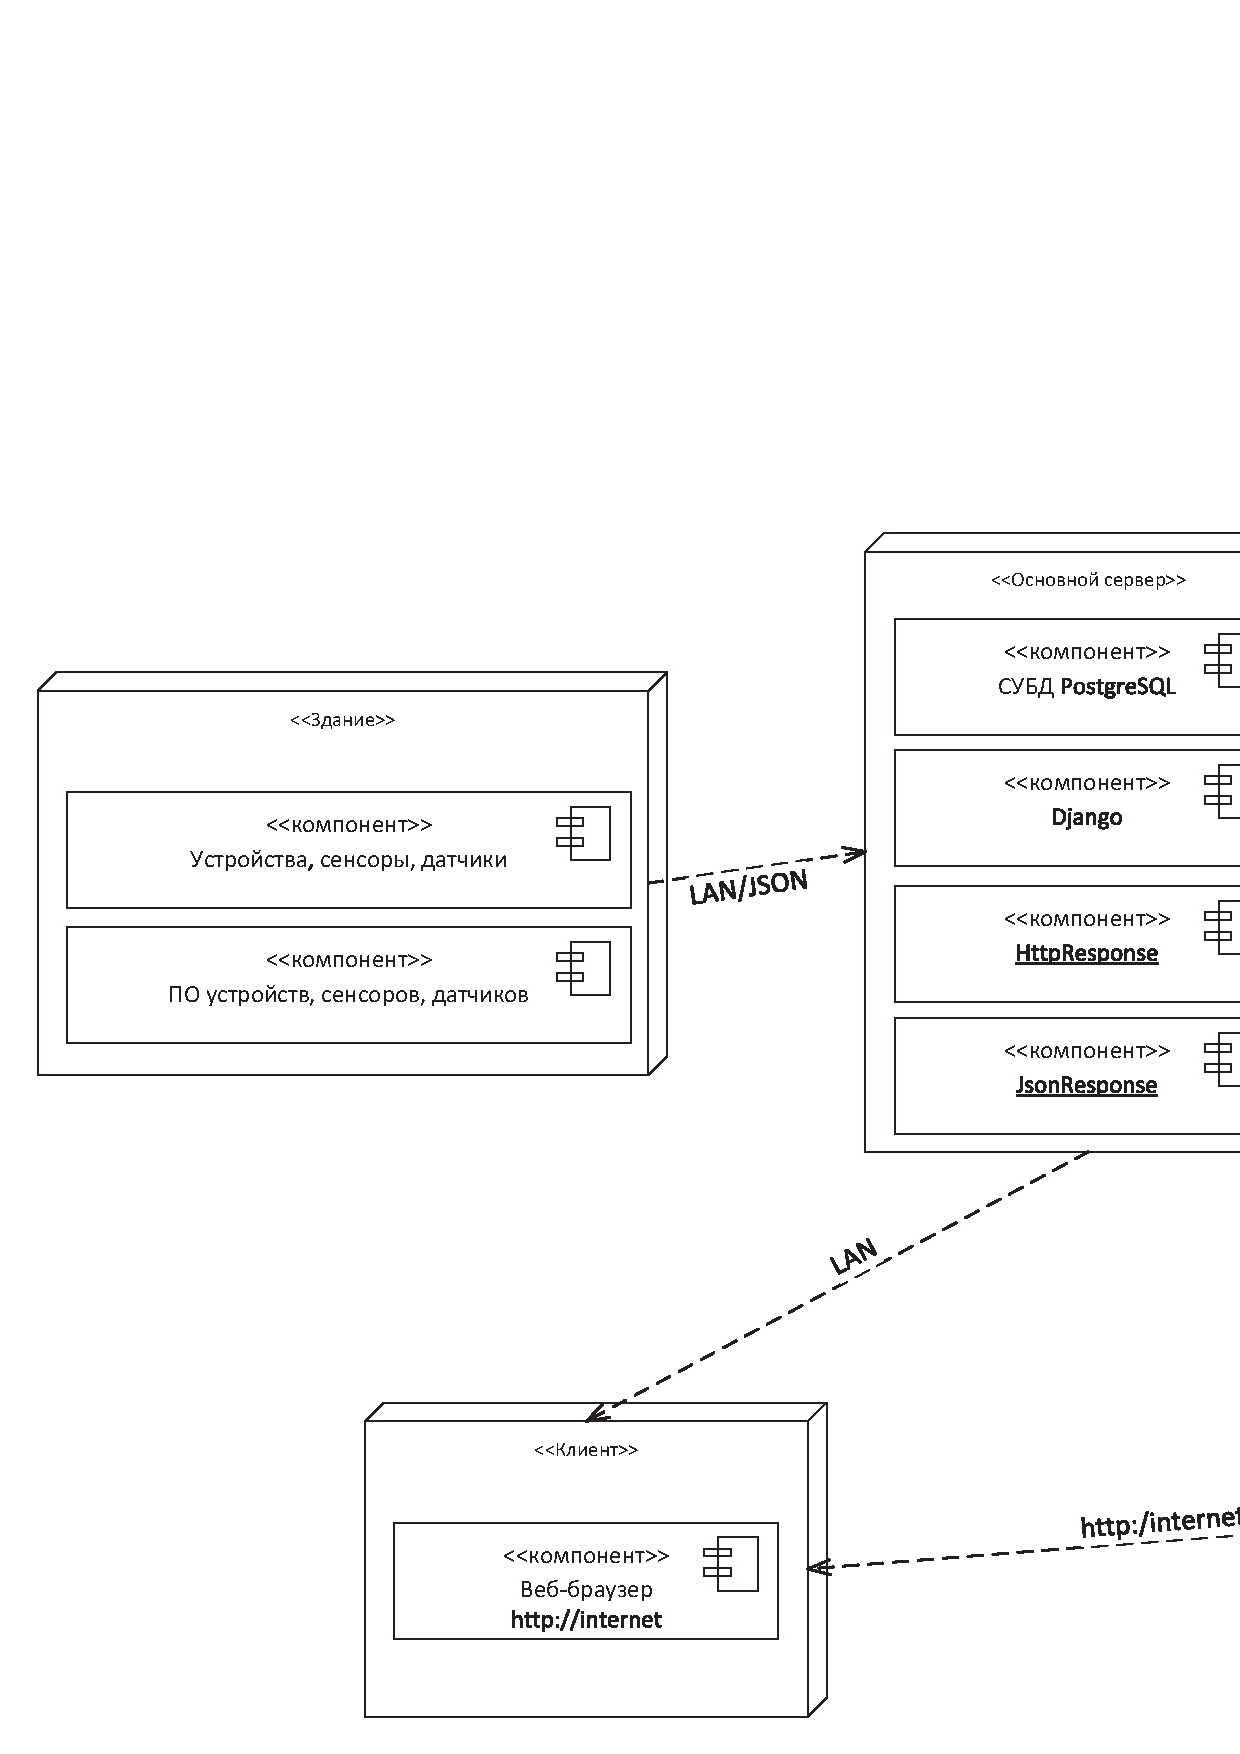
\includegraphics[width=0.82\linewidth]{place}
		\caption{Диаграмма размещения}
		\label{place:image}      
	\end{плакат}
\end{landscape}



\begin{enumerate}


\item {Сервер:}
\begin{itemize}
	\item {Описание:} Физический или виртуальный сервер, на котором размещена программно-информационная система. Сервер выполняет обработку запросов, взаимодействует с базой данных, и управляет основной логикой системы.
	\item {Размещение:} Сервер расположен в дата-центре компании и подключен к высокоскоростной сети интернета.
	\item {Компоненты:} Django приложение, бизнес-логика, веб-сервер.
\end{itemize}

\item {База данных:}
\begin{itemize}
	\item {Описание:} Хранилище данных, где сохраняются все необходимые для системы информационные записи. В данной системе используется реляционная база данных для хранения данных о компаниях, потреблении энергии, настройках и других сущностях.
	\item {Размещение:} Физически база данных размещена на сервере в дата-центре, обеспечивая быстрый доступ к данным.
	\item {Компоненты:} PostgreSQL (или другая СУБД), таблицы с данными.
\end{itemize}

\item Устройства сбора данных:
\begin{itemize}
\item  {Описание:} Физические устройства, установленные в зданиях, ответственные за сбор данных о потреблении энергии и внесение корректив в управление энергопотреблением в реальном времени. Компоненты включают в себя сенсоры, датчики влажности, температуры, освещенности и другие.
\item  {Размещение:} Сенсоры и датчики подключены к локальной сети в каждом здании компании, обеспечивая сбор данных в реальном времени.
\item  {Компоненты:} Сенсоры, датчики, средства сбора и передачи данных.
\item  {Сеть:} Устройства сбора данных подключены к локальной сети здания, обеспечивая передачу данных на сервер через сетевой протокол (например, TCP/IP). Данные могут быть переданы в формате JSON для удобства обработки на сервере.
\end{itemize}
	
\item Пользовательские устройства():
\begin{itemize}
	\item {Описание:} Пользовательские интерфейсы представлены на клиентских устройствах, таких как компьютеры, планшеты или мобильные устройства. Здесь пользователи могут взаимодействовать с системой, вводя данные или получая информацию.
	\item {Размещение:} Устройства клиентов находятся в офисах компаний, а также могут использоваться удаленные рабочие места.
	\item {Компоненты:} Браузеры (Google Chrome, Mozilla Firefox, Safari и др.), интерфейс пользователя.
\end{itemize}


\item Сетевые соединения, стрелки, обозначающие сетевые соединения между устройствами, чтобы показать, как данные передаются между ними.


\end{enumerate}

Диаграмма размещения демонстрирует (рис.~\ref{place:image}) , как каждый компонент системы взаимодействует друг с другом и как данные передаются между устройствами.


%\vspace{-8mm} % чтобы убрать пустую строку, которая осталась после переноса рисунка на следующую страницу
%\begin{figure}[ht]
%	\center{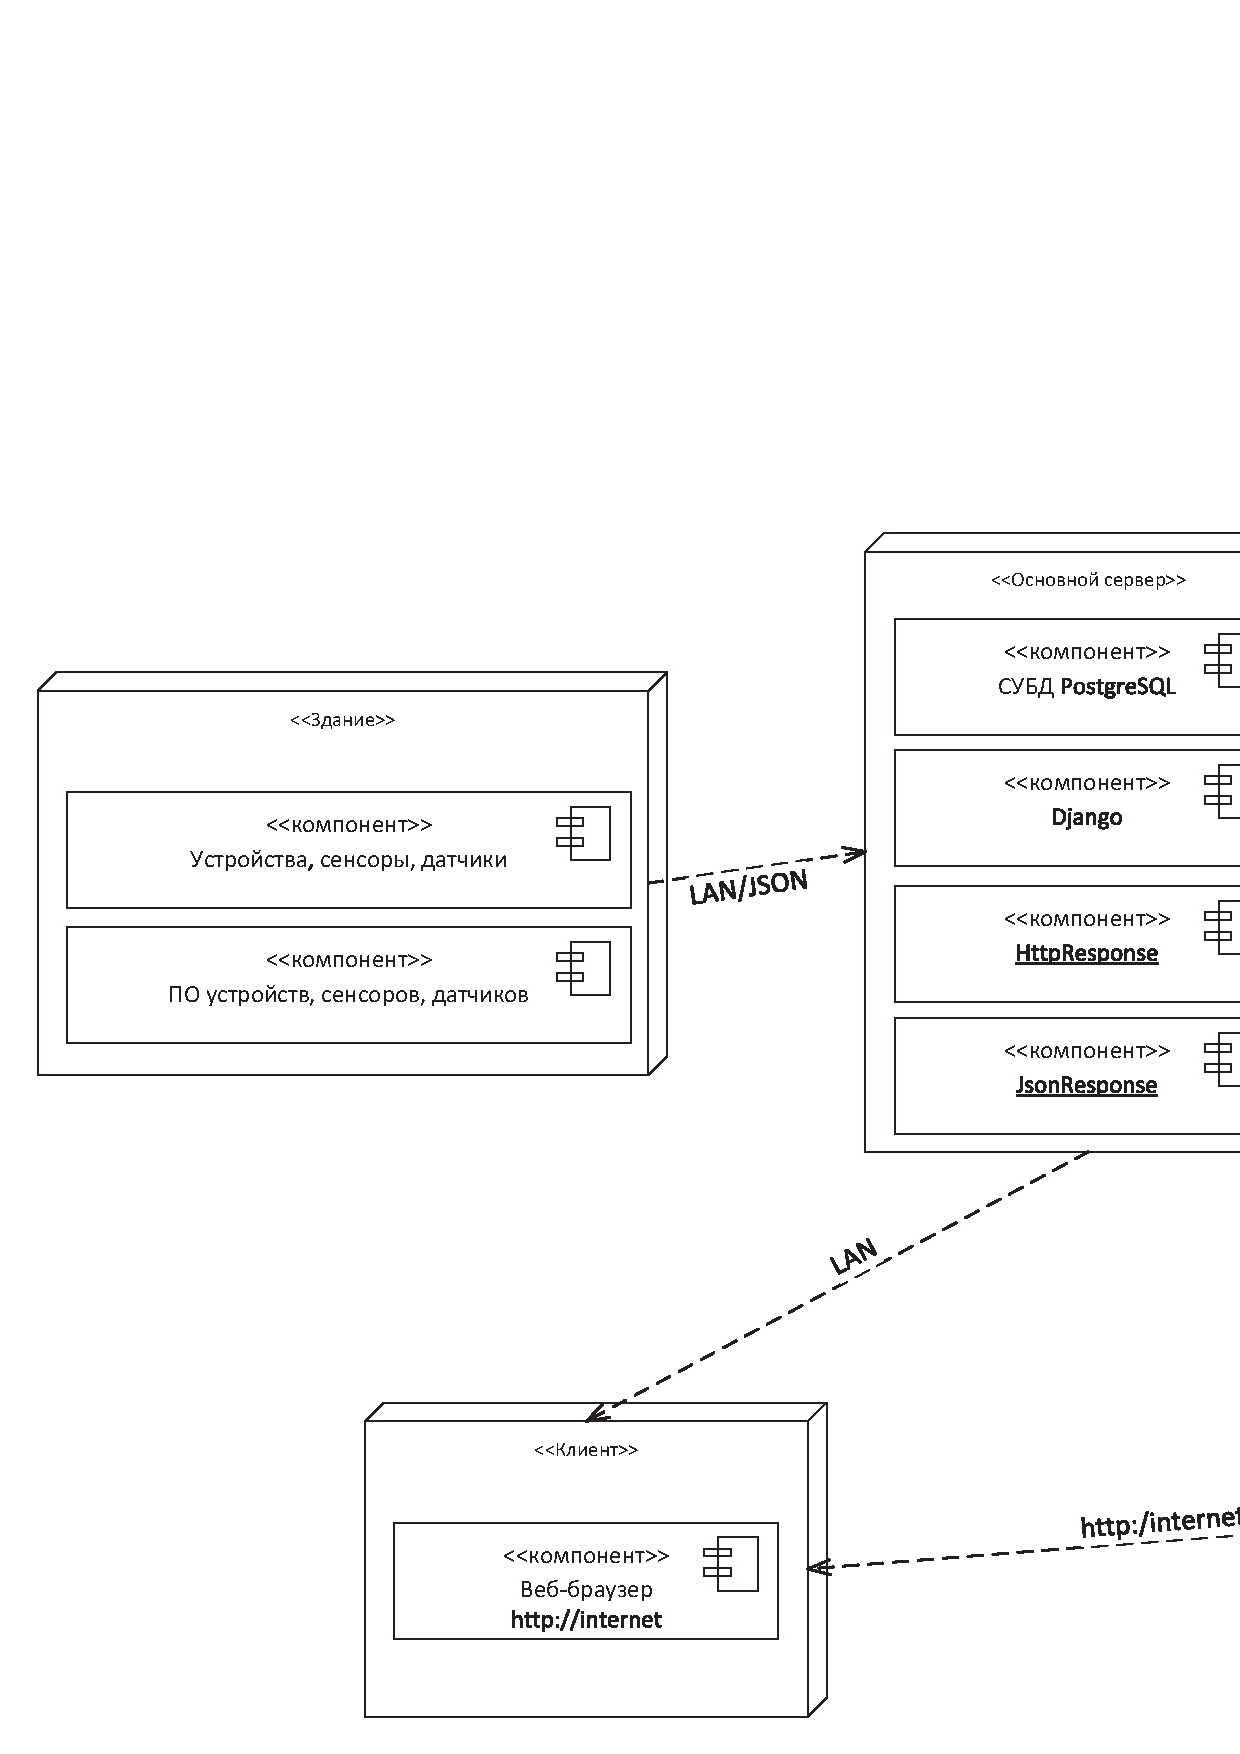
\includegraphics[width=0.9\linewidth]{place}}
%	\caption{Диаграмма размещения}
%	\label{place:image}
%\end{figure}



\subsection{Диаграмма классов}

Диаграмма классов представляет собой визуализацию структуры классов программной системы и их взаимосвязей. Ниже приведено описание основных классов системы "Программно-информационная система для управления энергопотреблением в зданиях".

Классы, представление классов с их атрибутами и методами:

\begin{enumerate}
	
\item {Класс <<EnergyConsumption>>:} Модель для учета потребленной энергии.
\begin{itemize}
	\item {Атрибуты:}  company, room, floor, date, consumption\_without\_an\_assistant, consumption\_with\_an\_assistant, total\_amount\_of\_electricity\_consumed\_without\_an\_assistant, total\_amount\_of \_electricity\_consumed\_with\_the\_assistant, total\_cost\_without\_an\_assistant, total\_cost\_with\_an\_assistant, humidity, temperature, illumination, motion.
	\item {Методы:} {\_\_str\_\_}.
\end{itemize}

\item {Класс <<InventoryItemsNumber>>:} Модель для представления предметов в помещении.
\begin{itemize}
	\item {Атрибуты:} name, room.
	\item {Методы:} \_\_str\_\_.
\end{itemize}

\item {Класс <<Company>>:} Модель для представления компаний.
\begin{itemize}
	\item {Атрибуты:} name, color, object, number-of-employees.
	\item {Методы:} \_\_str\_\_.
\end{itemize}

\item {Класс <<Floor>>:} Модель для представления этажей.
\begin{itemize}
	\item {Атрибуты:} number.
	\item {Методы:} \_\_str\_\_.
\end{itemize}

\item {Класс <<Electricity>>:} Модель для представления электроэнергии.
\begin{itemize}
	\item {Атрибуты:} price, volume.
	\item {Методы:} \_\_str\_\_.
\end{itemize}
\end{enumerate}

{Объяснение основных классов:}

\begin{itemize}
	
	\item {EnergyConsumption:} Этот класс предназначен для учета и хранения данных о потреблении энергии в зданиях. Атрибуты класса включают в себя информацию о компании, помещении, этаже, дате, количестве потребленной энергии с и без использования системы управления, общей стоимости, а также дополнительные параметры, такие как влажность, температура, освещенность и обнаружение движения.
	
	\item {Класс <<InventoryItemsNumber>>:} Данный класс предназначен для представления предметов, находящихся в конкретном помещении. Атрибуты класса включают в себя название предмета и ссылку на помещение, где он находится. 
	
	\item {Класс <<Company>>:} Этот класс используется для представления компаний, использующих систему управления энергопотреблением. Атрибуты класса включают в себя название компании, цвет для визуализации, тип объекта компании и количество сотрудников.
	
	\item {Класс <<Floor>>:} Класс предназначен для хранения информации об этажах здания. Атрибуты класса включают в себя номер этажа.
	
	\item {Класс <<Electricity>>:} Данный класс используется для представления электроэнергии, собираемой и потребляемой системой. Атрибуты класса включают в себя цену за единицу электроэнергии и объем потребленной энергии.

\end{itemize}

Диаграмма классов представлена на рисунке ~\ref{classd111:image}, представляющее основные модели данных в вашем проекте на Django.


%Диаграмма классов представлена на рисунках ~\ref{classd1:image} - ~\ref{classd2:image}, %представляющая основные модели данных в вашем проекте на Django.

%\begin{figure}[ht]
%	\center{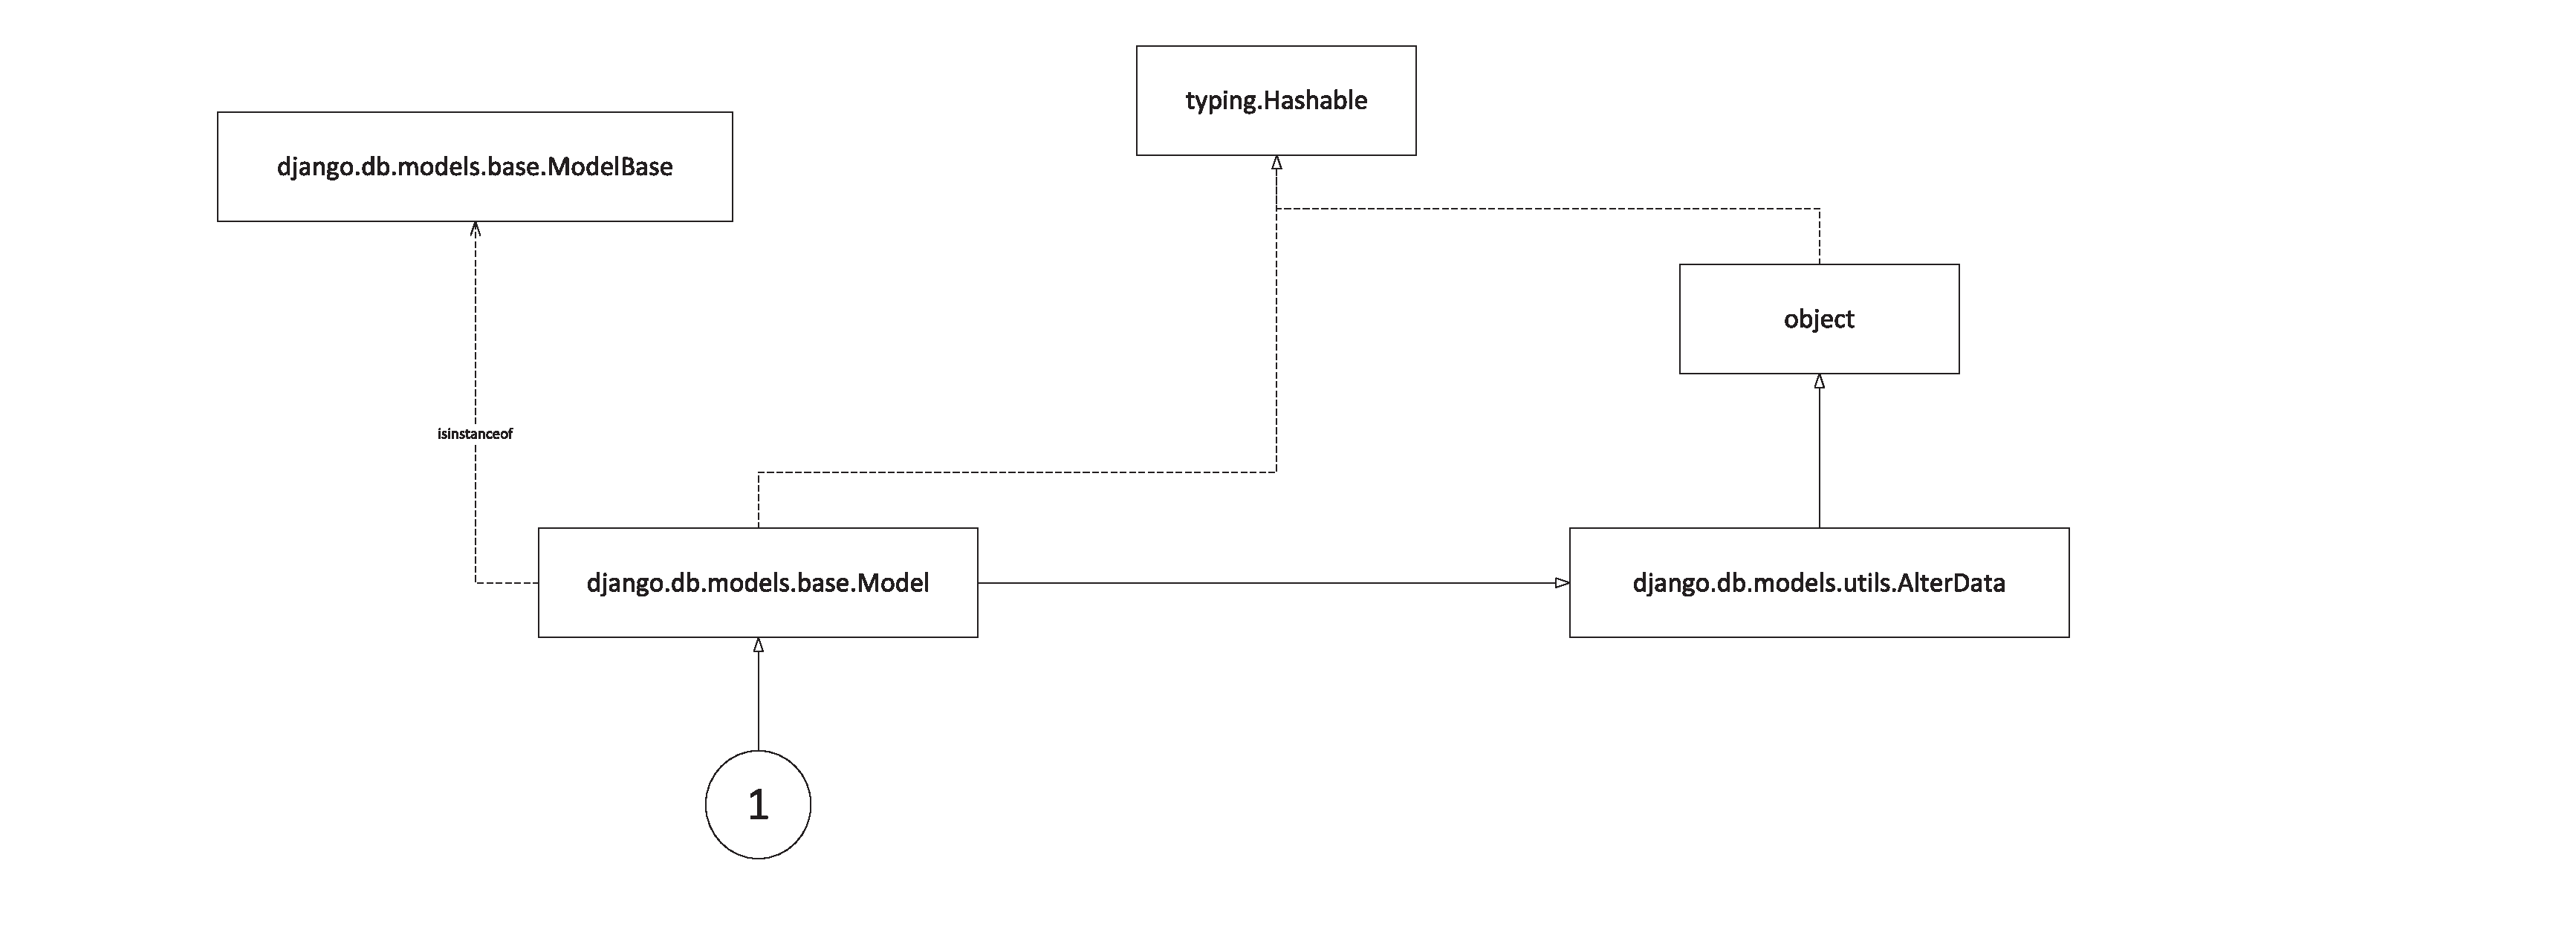
\includegraphics[width=1\linewidth]{classd1}}
%	\caption{Диаграмма классов}
%	\label{classd1:image}
%\end{figure}

%\newpage

%\begin{figure}[ht]
%	\center{\includegraphics[width=0.9\linewidth]{classd2}}
%	\caption{Диаграмма классов}
%	\label{classd2:image}
%\end{figure}


\begin{landscape}
	
	\begin{плакат}
		\includegraphics[width=0.82\linewidth]{classd111}
		\caption{Диаграмма классов}
		\label{classd111:image}      
	\end{плакат}
\end{landscape}



\newpage

\subsection{Содержание информационных блоков. Основные сущности}

Проанализировав требования, можно выделить несколько основных сущностей:

\begin{itemize}
	\item "<Потребление энергии">;
	\item "<Помещения">;
	\item "<Компании">;
	\item "<Этажи">;
	\item "<Предметы инвентаризации">;
	\item "<Электроэнергия">.
\end{itemize}

Сущность, отражающая данные о потреблении энергии компаниями на различных этажах и в разных помещениях. В состав сущности "<Потребление энергии"> можно включить атрибуты, представленные в таблице \ref{potrenergy:table}.

\begin{xltabular}{\textwidth}{|p{4cm}|l|p{1.7cm}|X|}
	\caption{Атрибуты сущности "<Потребление энергии">\label{potrenergy:table}}\\ \hline
	\centrow Поле & \centrow Тип & \centrow Обяза\-тельное & \centrow Описание \\ \hline
	\endfirsthead
	\continuecaption{Продолжение таблицы \ref{potrenergy:table}}
	\centrow Поле & \centrow Тип & \centrow Обяза\-тельное & \centrow Описание \\ \hline
	\finishhead
	company & ForeignKey(Company) & Да & Компания, потребляющая энергию. \\ \hline
	room & ForeignKey(Room) & Нет & Помещение, в котором измеряется потребление. \\ \hline
	floor & ForeignKey(Floor) & Нет & Этаж, на котором расположено помещение. \\ \hline
	date & DateField & Да & Дата, когда было измерено потребление. \\ \hline
	consumption-without-an-assistant & JSONField & Да & Потребление электроэнергии без использования умного помощника. \\ \hline
	consumption-with-an-assistant & JSONField & Да & Потребление электроэнергии с использованием умного помощника. \\ \hline
	total-amount-without-an-assistant & FloatField & Да & Общее количество потребляемой электричества без использования помощника. \\ \hline
	total-amount-with-the-assistant & FloatField & Да & Общее количество электричества, потребляемого с использованием помощника. \\ \hline
	total-cost-without-an-assistant & JSONField & Да & Общая стоимость потребления без использования помощника.\\ \hline
	total-cost-with-an-assistant & JSONField & Да & Общая стоимость потребления с использованием помощника. \\ \hline
	humidity & JSONField & Да & Значение влажности.\\ \hline
	temperature & JSONField & Да & Значение температуры. \\ \hline
	illumination & JSONField & Да & Значение освещенности.\\ \hline
	motion & JSONField & Да & Наличие движения.
\end{xltabular}
 
Сущность, описывающая различные помещения на этажах компаний. В состав сущности "<Помещения"> можно включить атрибуты, представленные в таблице \ref{room:table}.

\begin{xltabular}{\textwidth}{|p{4cm}|l|p{1.7cm}|X|}
	\caption{Атрибуты сущности "<Помещения">\label{room:table}}\\ \hline
	\centrow Поле & \centrow Тип & \centrow Обяза\-тельное & \centrow Описание \\ \hline
	\endfirsthead
	\continuecaption{Продолжение таблицы \ref{room:table}}
	\centrow Поле & \centrow Тип & \centrow Обяза\-тельное & \centrow Описание \\ \hline
	\finishhead
		name & CharField & Да & Название помещения.\\ \hline
		floor & ForeignKey(Floor) & Да & Этаж, на котором расположено помещение.
\end{xltabular}
 
Сущность, представляющая информацию о компаниях, потребляющих энергию. В состав сущности "<Компании"> можно включить атрибуты, представленные в таблице \ref{company:table}.

\begin{xltabular}{\textwidth}{|p{4cm}|l|p{1.7cm}|X|}
	\caption{Атрибуты сущности "<Компании">\label{company:table}}\\ \hline
	\centrow Поле & \centrow Тип & \centrow Обяза\-тельное & \centrow Описание \\ \hline
	\endfirsthead
	\continuecaption{Продолжение таблицы \ref{company:table}}
	\centrow Поле & \centrow Тип & \centrow Обяза\-тельное & \centrow Описание \\ \hline
	\finishhead
		name & CharField & Да & Название компании.\\ \hline
		color & ForeignKey(Color) & Нет & Цвет, ассоциированный с компанией.\\ \hline
		object & ForeignKey(BuilderObject) & Да & Расположение компании.\\ \hline
		number-of-employees & CharField & Да & Количество сотрудников компании.
\end{xltabular}

 
Сущность, описывающая различные этажи в здании. В состав сущности "<Этажи"> можно включить атрибуты, представленные в таблице \ref{floor:table}.

\begin{xltabular}{\textwidth}{|p{4cm}|l|p{1.7cm}|X|}
	\caption{Атрибуты сущности "<Этажи">\label{floor:table}}\\ \hline
	\centrow Поле & \centrow Тип & \centrow Обяза\-тельное & \centrow Описание \\ \hline
	\endfirsthead
	\continuecaption{Продолжение таблицы \ref{floor:table}}
	\centrow Поле & \centrow Тип & \centrow Обяза\-тельное & \centrow Описание \\ \hline
	\finishhead
 		number & CharField & Да & Номер этажа.
\end{xltabular}

Сущность, отражающая предметы в помещении.В состав сущности "<Предметы инвентаризации"> можно включить атрибуты, представленные в таблице \ref{predmet:table}.

\begin{xltabular}{\textwidth}{|p{4cm}|l|p{1.7cm}|X|}
	\caption{Атрибуты сущности "<Предметы инвентаризации">\label{predmet:table}}\\ \hline
	\centrow Поле & \centrow Тип & \centrow Обяза\-тельное & \centrow Описание \\ \hline
	\endfirsthead
	\continuecaption{Продолжение таблицы \ref{predmet:table}}
	\centrow Поле & \centrow Тип & \centrow Обяза\-тельное & \centrow Описание \\ \hline
	\finishhead
		name & ForeignKey(InventoryItems) & Да & Предмет инвентаризации.\\ \hline
		room & ForeignKey(Room) & Да & Помещение, в котором размещается предмет. 
\end{xltabular}

 
Эти сущности предоставляют функционал для отслеживания и анализа потребления энергии, структуры помещений, информации о компаниях, этажах, предметах инвентаризации и стоимости электроэнергии.
